\documentclass[uplatex, dvipdfmx]{jsarticle}
\和暦
\usepackage[top=25truemm,bottom=25truemm,left=25truemm,right=25truemm]{geometry}
\usepackage{graphicx}
\usepackage{color}
\graphicspath{{./images/}}
\setcounter{tocdepth}{3} % show subsubsection in table of contents

% Title
\title{\huge 報告書}
\author{Lewis Hamilton}
\date{\today}

% Main Content
\begin{document}

% --------------------------------------------------------------------------------
\maketitle
\thispagestyle{empty}
\newpage

% --------------------------------------------------------------------------------
\tableofcontents % make content page
\newpage

% --------------------------------------------------------------------------------
\section{数式テスト}
inline 数式 : ${\rm x \times y = xy}$
通常数式
\begin{equation}
  x \times y = xy
\end{equation}
番号なし数式
\begin{eqnarray*}
  x \times y = xy
\end{eqnarray*}

% --------------------------------------------------------------------------------
\section{画像テスト}
\begin{figure}
  \centering
  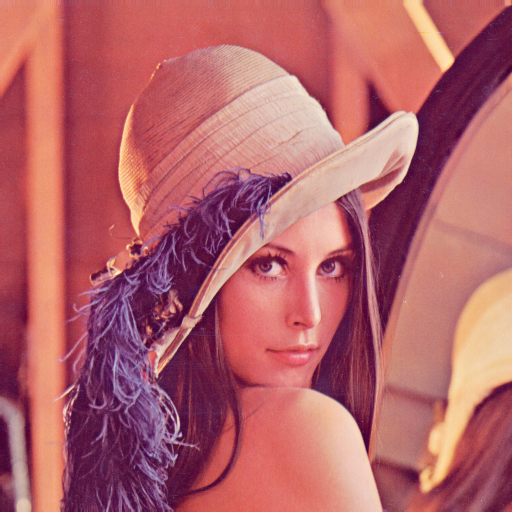
\includegraphics[width=0.95\textwidth]{Lenna.png}
  \caption{キャプション}
  \label{figure_label}
\end{figure}

%% \afterpage{\clearpage}

% --------------------------------------------------------------------------------
\input input_sample.tex

\end{document}
